\documentclass[tikz]{standalone}
\usepackage{amsmath}
\usepackage{tikz}

\begin{document}
	
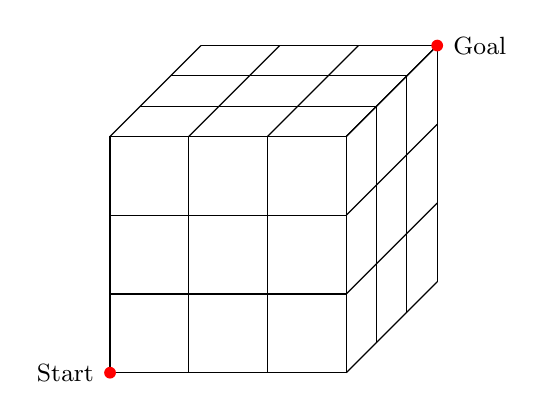
\begin{tikzpicture}

\pgfmathsetmacro{\N}{3}
\foreach \x in{0,...,\N}
{   \draw (0,\x ,\N) -- (\N,\x ,\N);
	\draw (\x ,0,\N) -- (\x ,\N,\N);
	\draw (\N,\x ,\N) -- (\N,\x ,0);
	\draw (\x ,\N,\N) -- (\x ,\N,0);
	\draw (\N,0,\x ) -- (\N,\N,\x);
	\draw (0,\N,\x ) -- (\N,\N,\x );
}
	
\node[circle, fill=red, inner sep=1.5pt,label=right:{\small Goal}] (start) at (\N,\N,0) {};
\node[circle, fill=red, inner sep=1.5pt,label=left:{\small Start}] (start) at (0,0,\N) {};	

\end{tikzpicture}
\end{document}
